
\begin{table*}
\centering \caption{We varied $T$, the expected number of topical relevance (rows), and the mean $\mu$ of Gaussian distribution used to generate understandability labels (columns). 
    A smaller $\mu$ means that easier to read documents are retrieved.
    We showed the average and standard deviation of each experiment. All numbers were multiplied by 100. }
\label{tab:simulations} \resizebox{1.\textwidth}{!}{ %
\begin{tabular}{cllllllllllll}
\toprule 
\multirow{2}{*}{$T$}  & \multicolumn{4}{c}{\textbf{Understandability $\mathcal{N}$(50,40)}} & \multicolumn{4}{c}{\textbf{Understandability $\mathcal{N}$(40,40)}} & \multicolumn{4}{c}{\textbf{Understandability $\mathcal{N}$(30,40)}}\tabularnewline
\cmidrule{2-13}
 & RBP  & uRBP  & $RBP_{u}$  & $H_{RBP}$  & RBP  & uRBP  & $RBP_{u}$  & $H_{RBP}$  & RBP  & uRBP  & $RBP_{u}$  & $H_{RBP}$ \tabularnewline
\midrule 
0.3 & 28$\pm$1 & 14$\pm$1 & 41$\pm$1 & 30$\pm$1 & 28$\pm$1 & 16$\pm$1 & 50$\pm$1 & 33$\pm$1 & 28$\pm$1 & 19$\pm$1 & 59$\pm$2 & 35$\pm$1\tabularnewline
0.4 & 38$\pm$2 & 19$\pm$1 & 41$\pm$1 & 36$\pm$1 & 38$\pm$2 & 21$\pm$1 & 50$\pm$1 & 39$\pm$1 & 38$\pm$2 & 25$\pm$1 & 60$\pm$1 & 43$\pm$1\tabularnewline
0.5 & 47$\pm$1 & 24$\pm$1 & 41$\pm$1 & 40$\pm$1 & 47$\pm$1 & 26$\pm$1 & 49$\pm$1 & 45$\pm$1 & {\cellcolor{yellow!25}} 47$\pm$1 & {\cellcolor{yellow!25}} 30$\pm$1 & {\cellcolor{yellow!25}} 60$\pm$1 & {\cellcolor{yellow!25}} 49$\pm$1\tabularnewline
0.6 & 56$\pm$1 & 28$\pm$1 & 41$\pm$1 & 44$\pm$1 & {\cellcolor{blue!25}}56$\pm$1 & {\cellcolor{blue!25}}32$\pm$1 &  {\cellcolor{blue!25}}49$\pm$2 & {\cellcolor{blue!25}}49$\pm$1 & 56$\pm$1 & 37$\pm$1 & 60$\pm$1 & 55$\pm$1\tabularnewline
0.7 & 65$\pm$1 & 33$\pm$1 & 42$\pm$1 & 48$\pm$1 & 65$\pm$1 & 37$\pm$1 & 49$\pm$1 & 53$\pm$1 & 65$\pm$1 & 42$\pm$1 & 60$\pm$1 & 60$\pm$1\tabularnewline
\bottomrule
\end{tabular}} 
\end{table*}




\section{Comparing frameworks Through System Simulations}
\label{sec:simulations}

To understand the behaviour of UBIRE and $MM$ when facing different IR systems, we first employed synthetic systems so as to have a fine-grained control over our experiments. This allowed to know a priori what has changed between two system instances and study the effect these changes had on evaluation. In our experiments, along with topicality, we considered understandability, leaving the (trivial) extension to other dimensions to later work. 
In the following simulations we controlled the amount of topical documents and understandable documents retrieved. We did so by following this two-phase procedure:

\begin{enumerate}
\item \textbf{Topicality Phase:} we controlled the amount of topical documents in a simulated run using a random variable $T$, $0 \le T \le 1$. 
We constructed a synthetic run by drawing a real number $N_i$, $0 \le N_i \le 1$, for each position $i$ in a ranking. If $N_i \le T$, we marked the document at position $i$ as relevant, otherwise, we marked it as not relevant. It is expected that a run generated with $T=0.1$ has 10\% of the documents assessed as relevant (90\% as non-relevant), while a run with $T=0.5$ has as many relevant as non-relevant documents. 

\item \textbf{Understandability Phase:}  we controlled the level of understandability of the documents in a synthetic run. In order to create and control the randomness of our synthetic systems, we generated understandability labels using a Gaussian distribution with pre-defined mean $\mu$ and variance $\sigma$. 
As previously done in consumer health search collections~\cite{clefIR16,clefIR17}, we forced the understandability labels to be in the interval $[0,100]$. 
We fixed a relatively large variance, $\sigma=40$, to mimic results of previous collections in which the understandability labels had a large variance \cite{clefIR16}, and we varied the mean $\mu$ of the Gaussian from 0 to 100. Figure~\ref{fig:gaussians} shows the expected label distribution for $\mu=20, 50, 80$, i.e., $\mathcal{N}(20, 40)$, $\mathcal{N}(50, 40)$ and $\mathcal{N}(80, 40)$.
In Figure~\ref{fig:gaussians} we also included the threshold U used to compute $RBP_u$ (Section~\ref{sec:extension}).
\end{enumerate}
%
%We executed these two phases in succession. In total, we generated 1,000 runs for each value of T (topicality phase) and $\mu$ value (understandability phase). 
We executed these two phases in succession. In total, we generated 1,000 runs for each value of T and $\mu$. 

\begin{figure}[t!]
  \centering
   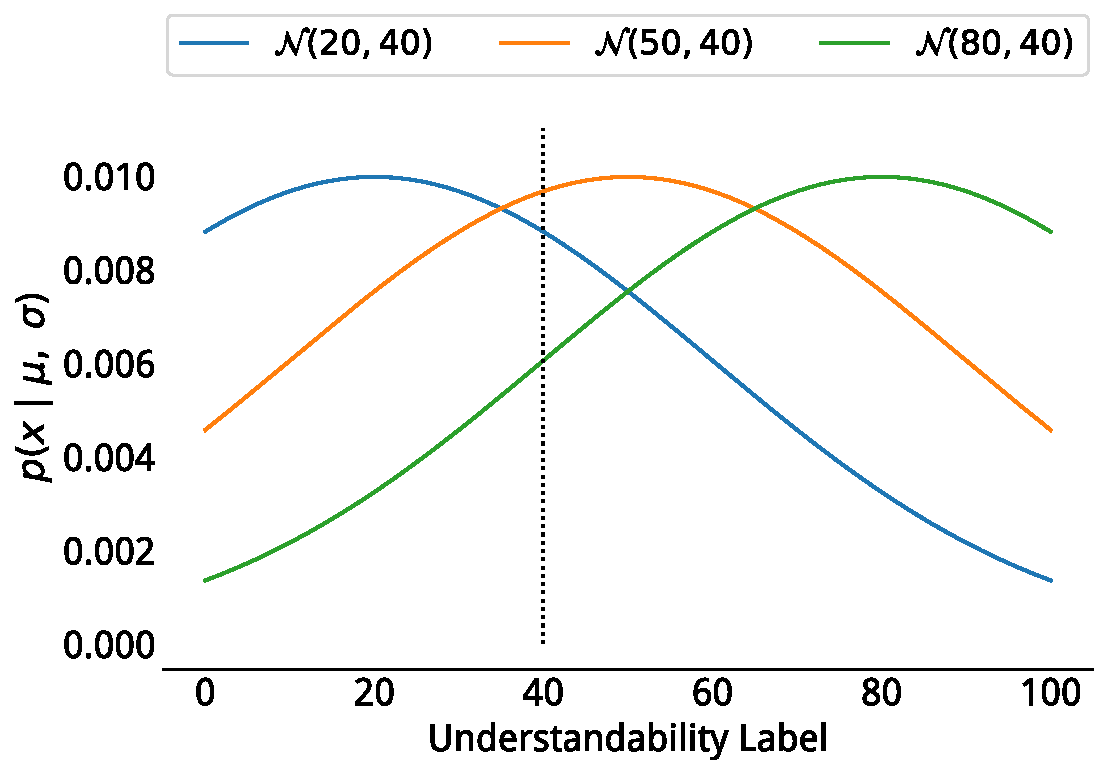
\includegraphics[width=0.30\textwidth]{figs/gaussians2}
    \vspace{-.2cm}
    \caption{Gaussian distribution for different $\mu$: higher $\mu$ generates higher understandability labels (more difficult documents were retrieved). Here, only documents with understandability lower than 40 are considered easy-to-understand (threshold shown as dotted line). \vspace{-16pt}}
  \label{fig:gaussians}
\end{figure}

We calculated $uRBP$ (using UBIRE) and $MM_{RBP}$ for each synthetic system.
%The average result of the synthetic runs is shown in Table~\ref{tab:simulations}. Each row shows the results of simulations with different values for $T$, i.e., different expected number of topical documents retrieved.
%Each row shows the results of simulations with different values for $T$, i.e., different expected number of topical documents retrieved.
%We varied $\mu$ which was used to create the understandability labels, and show the results for $\mu = 50, 40, 30$.
Table~\ref{tab:simulations} shows the average result for different values of $T$ (rows), i.e., different expected number of topical documents retrieved, and values of $\mu$ (cols), i.e., different understandability distributions.
A smaller $\mu$ means that more understandable documents were retrieved. The results show that as the expected number of topical documents ($T$) increases, $RBP$ increases. Likewise, $uRBP$ increases, as it is bounded by topical relevance.
In turn, increasing $T$ has no effect on $RBP_u$, but increases $MM_{RBP}$, as it is also directly dependant on $RBP$. When the number of understandable documents retrieved is increased (i.e., $\mu$ decreased ), $RBP$ stays constant, as it does not measure how understandable documents are.
In turn, $uRBP$, $RBP_u$ and $MM_{RBP}$ increase. 
These are the expected behaviours of the considered measures. % aforementioned metrics and only shows that our simulated runs produce sane results.

We further focused our attention to the results of specific experiments highlighted in blue and yellow in Table~\ref{tab:simulations}. These cases simulated an initial system S1 that exhibited the results in blue (condition $T=0.6$ and $\mathcal{N}(40,40)$) being modified to improve the understandability of retrieved documents ($\mathcal{N}(30,40)$) at the expenses of topicality ($T=0.5$), producing a new system S2. The effectiveness of S2 is highlighted in yellow. 

If $RBP$ and $uRBP$ were used to decide whether S2 should be preferred over the initial system S1, then S2 would be discarded and S1 preferred, as S2 produced a $16\%$ reduction in $RBP$ and a $6\%$ reduction in $uRBP$. With these results, an IR researcher would conclude that the modifications in S2 did not pay off.

If $MM_{RBP}$ was used instead, the IR researcher would have been able to gain more insights about system effectiveness and the trade-off between understandability and topicality. To use $MM_{RBP}$, $RBP_t$ ($=RBP$) and $RBP_u$ needed to be computed. Between S1 and S2, there was a decrease in $RBP_t$ of $16\%$; but conversely $RBP_u$ increased by $20\%$: this clearly allows the trade-off between topicality and understandability to be gauged. 

When $RBP$ and $uRBP$ were combined within $MM_{RBP}$, if both dimensions were given equal weight, then systems S1 and S2 obtained the same $MM_{RBP}$. Note that $MM$ can be adapted to specific circumstances: if topicality is more important than understandability, then the weights of each dimension can be changed accordingly in the harmonic mean computation. 

%%%%%%%%%%%%%%%%%%%%%%%%%%%%%%%%%%%%%%%%%%%%%%%%%%%%%%%%%%%%%%%%%%%%%%%%%%%%%%%%%%%%%%%%%%%%%%%%%%%%%%%%%%%%%%%%%%%%%%%%%%%%%%%%
%%%%%%%%%%%%%%%%%%%%%%%%%%%%%%%%%%%%%%%%%%%%%%%%%%%%%%%%%%%%%%%%%%%%%%%%%%%%%%%%%%%%%%%%%%%%%%%%%%%%%%%%%%%%%%%%%%%%%%%%%%%%%%%%
%%%%%%%%%%%%%%%%%%%%%%%%%%%%%%%%%%%%%%%%%%%%%%%%%%%%%%%%%%%%%%%%%%%%%%%%%%%%%%%%%%%%%%%%%%%%%%%%%%%%%%%%%%%%%%%%%%%%%%%%%%%%%%%%
%%%%%%%%%%%%%%%%%%%%%%%%%%%%%%%%%%%%%%%%%%%%%%%%%%%%%%%%%%%%%%%%%%%%%%%%%%%%%%%%%%%%%%%%%%%%%%%%%%%%%%%%%%%%%%%%%%%%%%%%%%%%%%%%

